% Options for packages loaded elsewhere
% Options for packages loaded elsewhere
\PassOptionsToPackage{unicode}{hyperref}
\PassOptionsToPackage{hyphens}{url}
%
\documentclass[
  english,
  russian,
  12pt,
  a4paper,
  DIV=11,
  numbers=noendperiod]{scrreprt}
\usepackage{xcolor}
\usepackage{amsmath,amssymb}
\setcounter{secnumdepth}{5}
\usepackage{iftex}
\ifPDFTeX
  \usepackage[T1]{fontenc}
  \usepackage[utf8]{inputenc}
  \usepackage{textcomp} % provide euro and other symbols
\else % if luatex or xetex
  \usepackage{unicode-math} % this also loads fontspec
  \defaultfontfeatures{Scale=MatchLowercase}
  \defaultfontfeatures[\rmfamily]{Ligatures=TeX,Scale=1}
\fi
\usepackage{lmodern}
\ifPDFTeX\else
  % xetex/luatex font selection
\fi
% Use upquote if available, for straight quotes in verbatim environments
\IfFileExists{upquote.sty}{\usepackage{upquote}}{}
\IfFileExists{microtype.sty}{% use microtype if available
  \usepackage[]{microtype}
  \UseMicrotypeSet[protrusion]{basicmath} % disable protrusion for tt fonts
}{}
\usepackage{setspace}
% Make \paragraph and \subparagraph free-standing
\makeatletter
\ifx\paragraph\undefined\else
  \let\oldparagraph\paragraph
  \renewcommand{\paragraph}{
    \@ifstar
      \xxxParagraphStar
      \xxxParagraphNoStar
  }
  \newcommand{\xxxParagraphStar}[1]{\oldparagraph*{#1}\mbox{}}
  \newcommand{\xxxParagraphNoStar}[1]{\oldparagraph{#1}\mbox{}}
\fi
\ifx\subparagraph\undefined\else
  \let\oldsubparagraph\subparagraph
  \renewcommand{\subparagraph}{
    \@ifstar
      \xxxSubParagraphStar
      \xxxSubParagraphNoStar
  }
  \newcommand{\xxxSubParagraphStar}[1]{\oldsubparagraph*{#1}\mbox{}}
  \newcommand{\xxxSubParagraphNoStar}[1]{\oldsubparagraph{#1}\mbox{}}
\fi
\makeatother


\usepackage{longtable,booktabs,array}
\newcounter{none} % for unnumbered tables
\usepackage{calc} % for calculating minipage widths
% Correct order of tables after \paragraph or \subparagraph
\usepackage{etoolbox}
\makeatletter
\patchcmd\longtable{\par}{\if@noskipsec\mbox{}\fi\par}{}{}
\makeatother
% Allow footnotes in longtable head/foot
\IfFileExists{footnotehyper.sty}{\usepackage{footnotehyper}}{\usepackage{footnote}}
\makesavenoteenv{longtable}
\usepackage{graphicx}
\makeatletter
\newsavebox\pandoc@box
\newcommand*\pandocbounded[1]{% scales image to fit in text height/width
  \sbox\pandoc@box{#1}%
  \Gscale@div\@tempa{\textheight}{\dimexpr\ht\pandoc@box+\dp\pandoc@box\relax}%
  \Gscale@div\@tempb{\linewidth}{\wd\pandoc@box}%
  \ifdim\@tempb\p@<\@tempa\p@\let\@tempa\@tempb\fi% select the smaller of both
  \ifdim\@tempa\p@<\p@\scalebox{\@tempa}{\usebox\pandoc@box}%
  \else\usebox{\pandoc@box}%
  \fi%
}
% Set default figure placement to htbp
\def\fps@figure{htbp}
\makeatother



\ifLuaTeX
\usepackage[bidi=basic,shorthands=off,provide=*]{babel}
\else
\usepackage[bidi=default,shorthands=off,provide=*]{babel}
\fi
\ifLuaTeX
  \usepackage{selnolig} % disable illegal ligatures
\fi


\setlength{\emergencystretch}{3em} % prevent overfull lines

\providecommand{\tightlist}{%
  \setlength{\itemsep}{0pt}\setlength{\parskip}{0pt}}



 
\usepackage[style=gost-numeric,backend=biber,langhook=extras,autolang=other*]{biblatex}
\addbibresource{bib/cite.bib}

\usepackage[]{csquotes}

\usepackage{indentfirst}
\usepackage{float}
\floatplacement{figure}{H}
\IfFileExists{plex-otf.sty}{
  %% Full TeXlive
  \usepackage[
    % math,
    RM={Scale=0.94},SS={Scale=0.94},SScon={Scale=0.94},TT={Scale=MatchLowercase,FakeStretch=0.9},
    DefaultFeatures={Ligatures=Common}
  ]{plex-otf}
  % \usepackage[Scale=MatchUppercase]{juliamono}
}{
  %% TinyTeX
  \usepackage{libertine}
}
\KOMAoption{captions}{tableheading}
\makeatletter
\@ifpackageloaded{caption}{}{\usepackage{caption}}
\AtBeginDocument{%
\ifdefined\contentsname
  \renewcommand*\contentsname{Содержание}
\else
  \newcommand\contentsname{Содержание}
\fi
\ifdefined\listfigurename
  \renewcommand*\listfigurename{Список иллюстраций}
\else
  \newcommand\listfigurename{Список иллюстраций}
\fi
\ifdefined\listtablename
  \renewcommand*\listtablename{Список таблиц}
\else
  \newcommand\listtablename{Список таблиц}
\fi
\ifdefined\figurename
  \renewcommand*\figurename{Рисунок}
\else
  \newcommand\figurename{Рисунок}
\fi
\ifdefined\tablename
  \renewcommand*\tablename{Таблица}
\else
  \newcommand\tablename{Таблица}
\fi
}
\@ifpackageloaded{float}{}{\usepackage{float}}
\floatstyle{ruled}
\@ifundefined{c@chapter}{\newfloat{codelisting}{h}{lop}}{\newfloat{codelisting}{h}{lop}[chapter]}
\floatname{codelisting}{Список}
\newcommand*\listoflistings{\listof{codelisting}{Листинги}}
\makeatother
\makeatletter
\makeatother
\makeatletter
\@ifpackageloaded{caption}{}{\usepackage{caption}}
\@ifpackageloaded{subcaption}{}{\usepackage{subcaption}}
\makeatother
\usepackage{bookmark}
\IfFileExists{xurl.sty}{\usepackage{xurl}}{} % add URL line breaks if available
\urlstyle{same}
% fallback for those not using the hyperref driver hyperxmp:
\makeatletter
\@ifundefined{xmpquote}{\newcommand{\xmpquote}[1]{#1}}{}
\makeatother
\hypersetup{
  pdftitle={Лабораторная работа №1},
  pdfauthor={Альманасра Рами},
  pdflang={ru-RU},
  hidelinks,
  pdfcreator={LaTeX via pandoc}}


\title{Лабораторная работа №1}
\usepackage{etoolbox}
\makeatletter
\providecommand{\subtitle}[1]{% add subtitle to \maketitle
  \apptocmd{\@title}{\par {\large #1 \par}}{}{}
}
\makeatother
\subtitle{Установка и конфигурация операционной системы на виртуальную
машину}
\author{Альманасра Рами}
\date{}
\begin{document}
\maketitle

\renewcommand*\contentsname{Содержание}
{
\setcounter{tocdepth}{1}
\tableofcontents
}
\listoffigures
\listoftables

\setstretch{1.5}
\chapter{Цель
работы}\label{ux446ux435ux43bux44c-ux440ux430ux431ux43eux442ux44b}

Целью данной работы является приобретение практических навыков установки
операционной системы на виртуальную машину, настройки минимально
необходимых для дальнейшей работы сервисов.

\chapter{Задание}\label{ux437ux430ux434ux430ux43dux438ux435}

\begin{itemize}
\tightlist
\item
  Установить Linux (Rocky) на виртуальную машину VirtualBox.
\item
  Выполнить базовую конфигурацию системы и сетевых параметров.
\item
  Подготовить систему для выполнения последующих лабораторных работ.
\end{itemize}

\chapter{Теоретическое
введение}\label{ux442ux435ux43eux440ux435ux442ux438ux447ux435ux441ux43aux43eux435-ux432ux432ux435ux434ux435ux43dux438ux435}

Виртуализация позволяет запускать гостевые операционные системы в
изолированной среде на одном физическом компьютере. Для учебных задач
удобно использовать VirtualBox, который поддерживает создание
виртуальных дисков, настройку ресурсов и подключение ISO-образов для
установки ОС. После установки важно выполнить базовую настройку системы:
задать имя хоста, создать пользователя, настроить сеть и убедиться в
корректной работе окружения

\chapter{Выполнение лабораторной
работы}\label{ux432ux44bux43fux43eux43bux43dux435ux43dux438ux435-ux43bux430ux431ux43eux440ux430ux442ux43eux440ux43dux43eux439-ux440ux430ux431ux43eux442ux44b}

\section{Создание виртуальной
машины}\label{ux441ux43eux437ux434ux430ux43dux438ux435-ux432ux438ux440ux442ux443ux430ux43bux44cux43dux43eux439-ux43cux430ux448ux438ux43dux44b}

Открываем VirtualBox и создаём новую виртуальную машину Указываем имя
виртуальной машины, определяем тип операционной системы и указываем путь
к iso-образу (рис.~\ref{fig-001})

\begin{figure}

\centering{

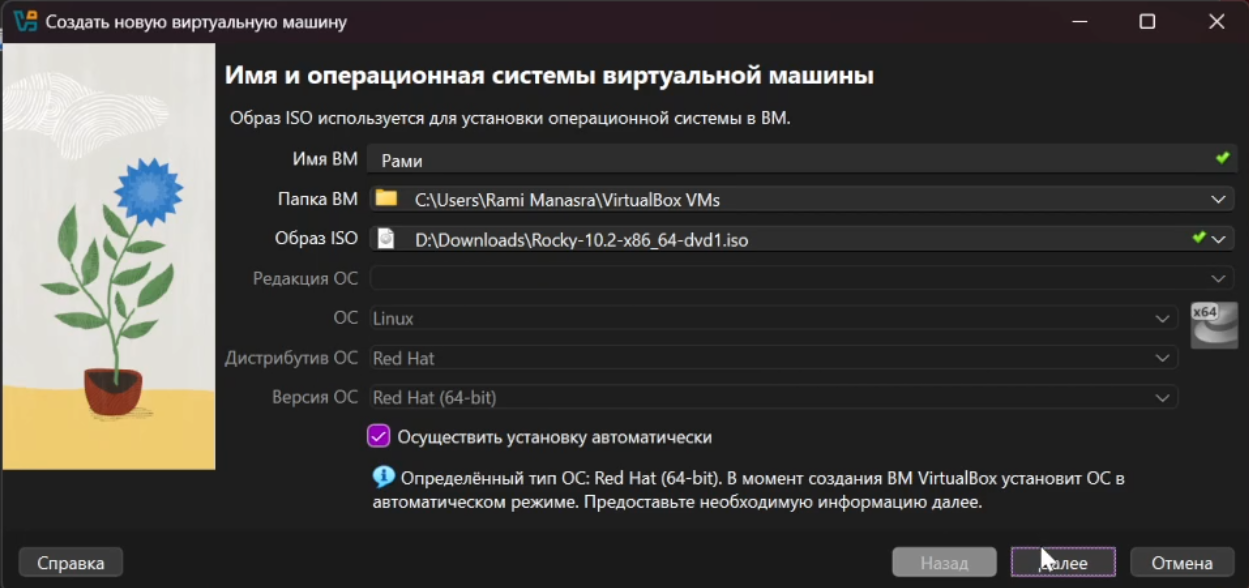
\includegraphics[width=0.7\linewidth,height=\textheight,keepaspectratio]{image/1.png}

}

\caption{\label{fig-001}Создание виртуальной машины}

\end{figure}%

Далее указываем размер оперативной памяти виртуальной машины - 2048 МБ,
число процессоров - 2 и задаём размер виртуального жёсткого диска - 40
ГБ (рис.~\ref{fig-002})

\begin{figure}

\centering{

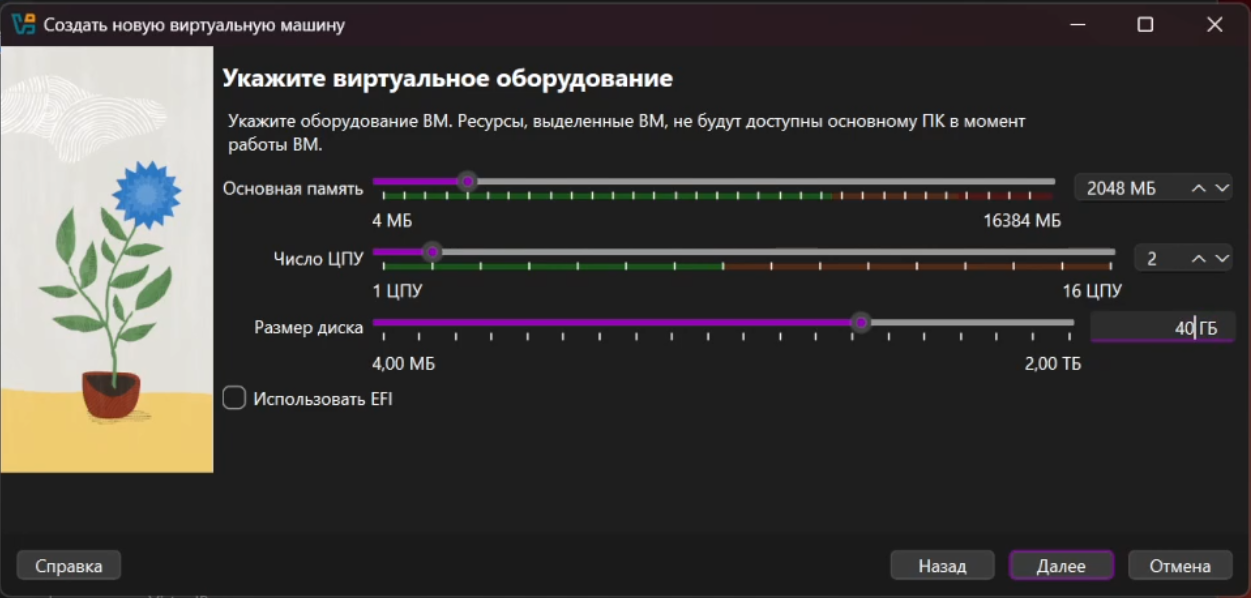
\includegraphics[width=0.7\linewidth,height=\textheight,keepaspectratio]{image/2.png}

}

\caption{\label{fig-002}Создание виртуалтной машины (2)}

\end{figure}%

\section{Установка операционной
системы}\label{ux443ux441ux442ux430ux43dux43eux432ux43aux430-ux43eux43fux435ux440ux430ux446ux438ux43eux43dux43dux43eux439-ux441ux438ux441ux442ux435ux43cux44b}

После запуска устанавливаем английский язык интерфейса
(рис.~\ref{fig-004})

\begin{figure}

\centering{

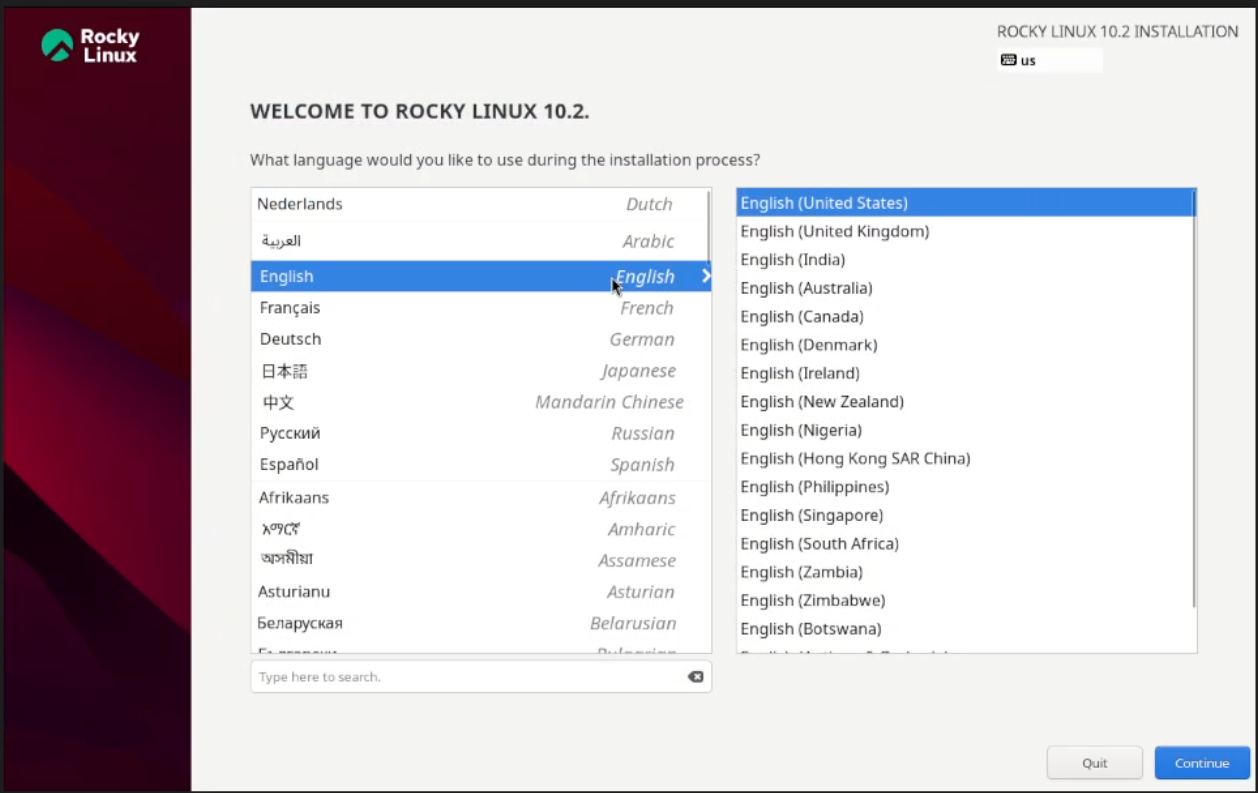
\includegraphics[width=0.7\linewidth,height=\textheight,keepaspectratio]{image/4.png}

}

\caption{\label{fig-004}Язык интерфейса - английский}

\end{figure}%

Добавляем русскую раскладку клавиатуры (рис.~\ref{fig-005})

\begin{figure}

\centering{

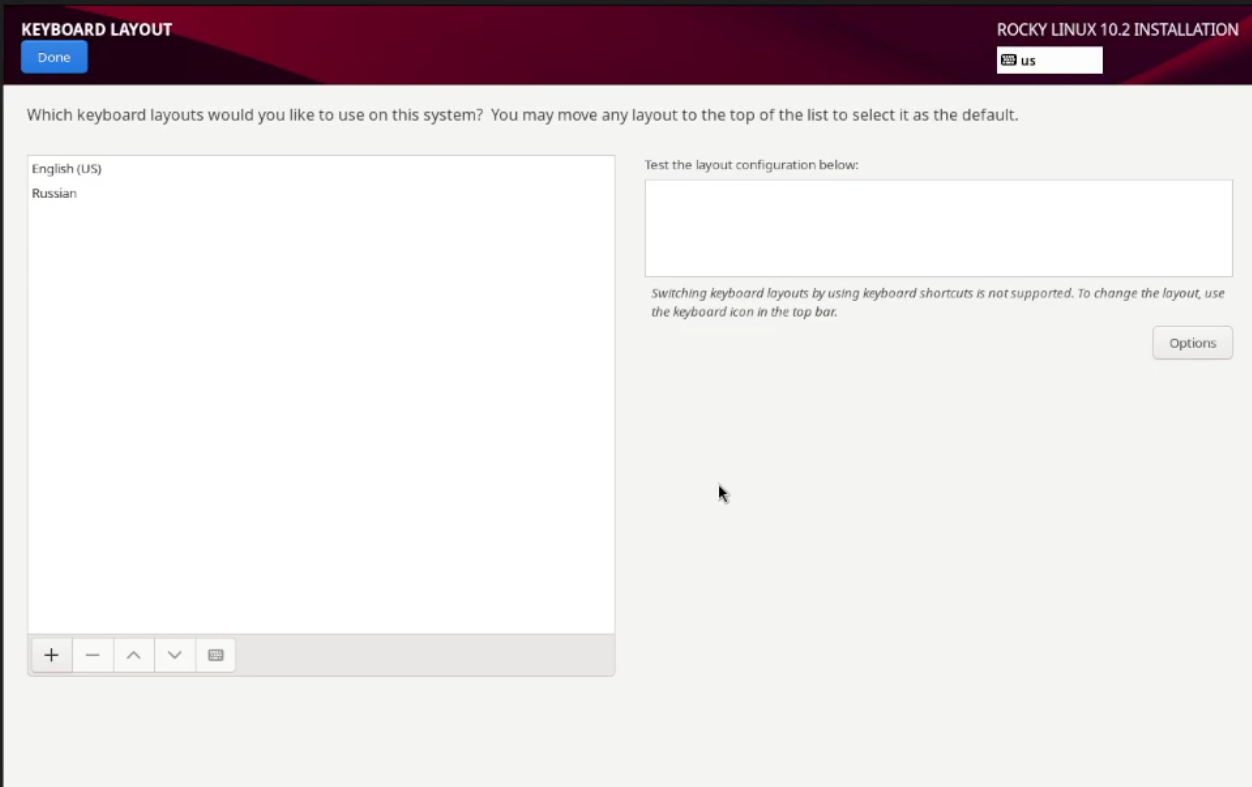
\includegraphics[width=0.7\linewidth,height=\textheight,keepaspectratio]{image/5.png}

}

\caption{\label{fig-005}Настройка раскладки клавиатуры}

\end{figure}%

В разделе выбора программ указываем в качестве базового окружения Server
with GUI, а в качестве дополнения --- Development Tools
(рис.~\ref{fig-007})

\begin{figure}

\centering{

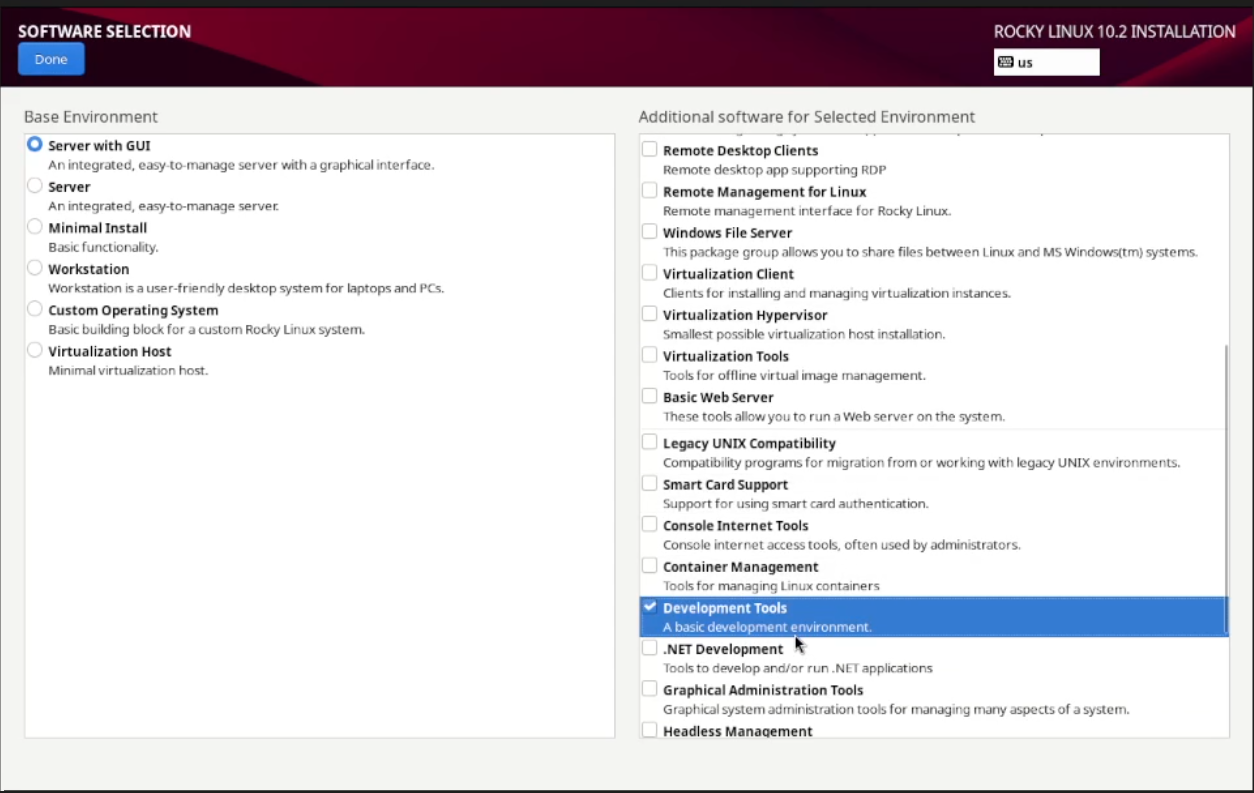
\includegraphics[width=0.7\linewidth,height=\textheight,keepaspectratio]{image/7.png}

}

\caption{\label{fig-007}Раздел выбора программ}

\end{figure}%

Далее отключаем KDUMP, а место установки ОС оставляем без изменения
(рис.~\ref{fig-008}), (рис.~\ref{fig-009})

\begin{figure}

\centering{

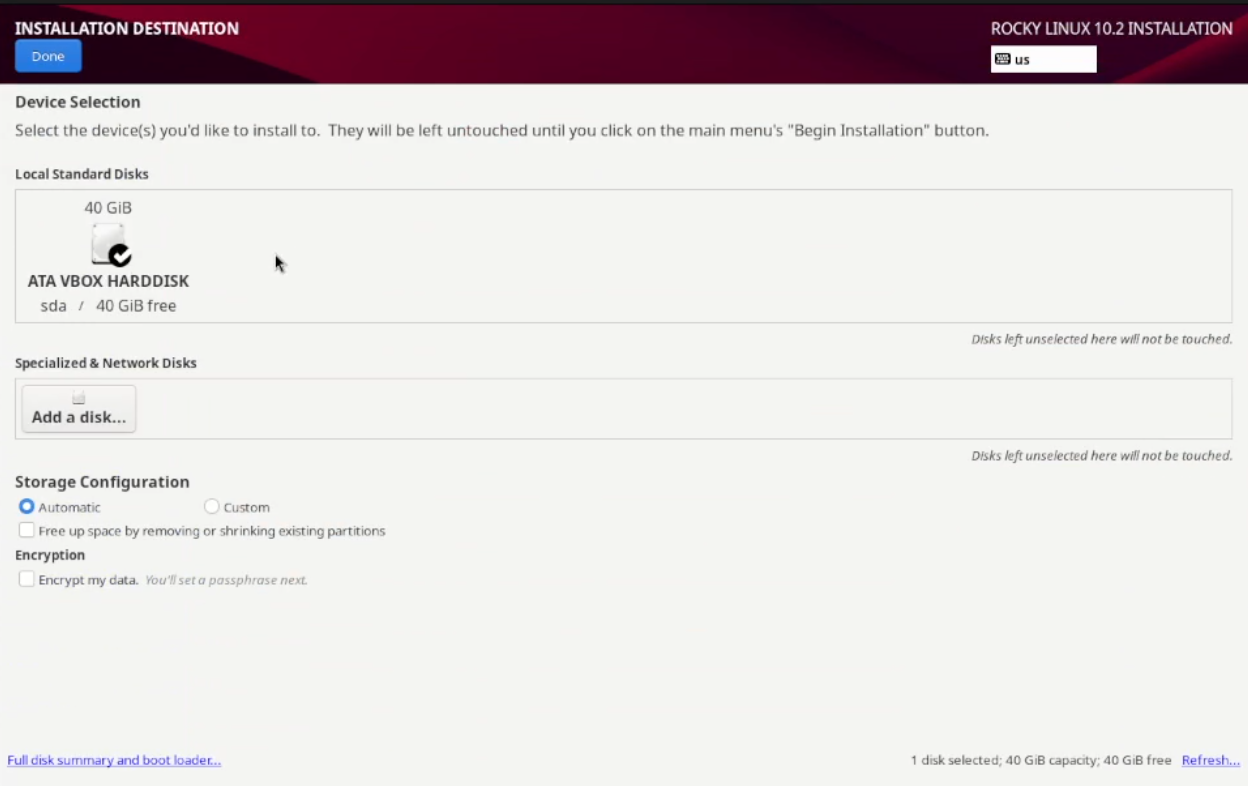
\includegraphics[width=0.7\linewidth,height=\textheight,keepaspectratio]{image/8.png}

}

\caption{\label{fig-008}Место установки ОС}

\end{figure}%

\begin{figure}

\centering{

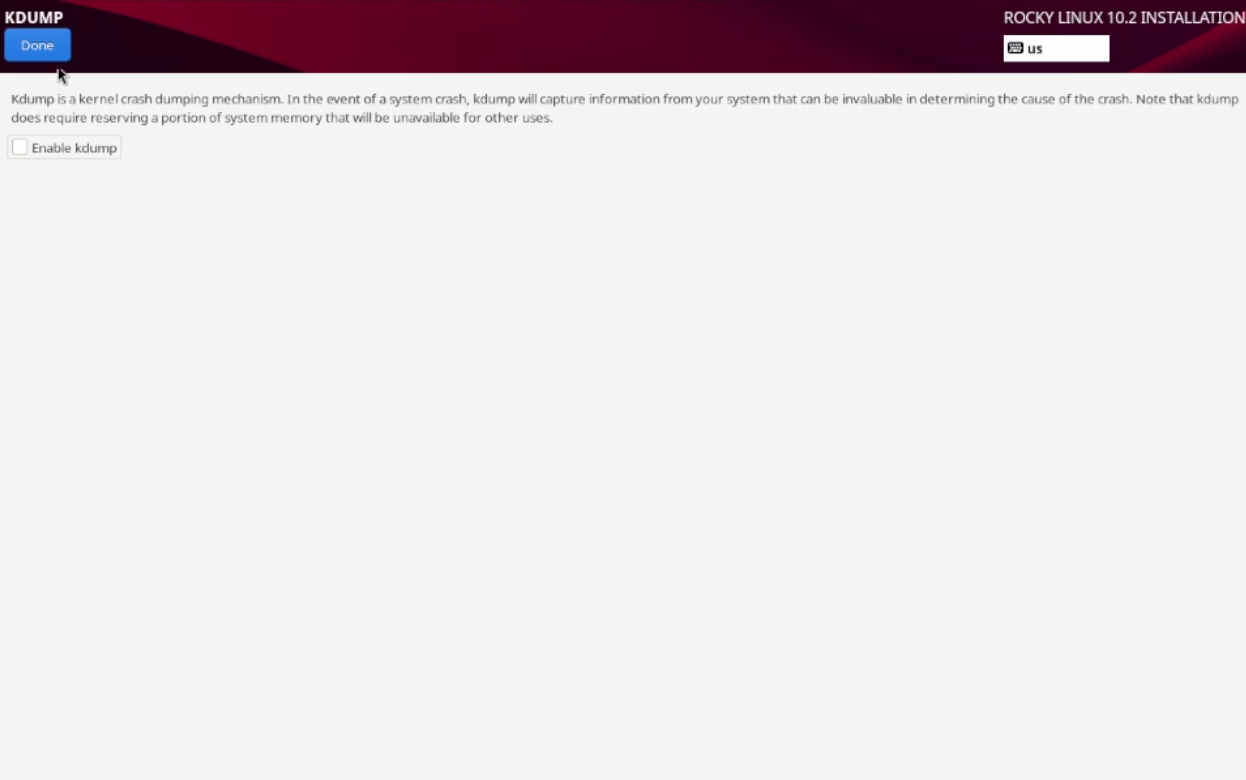
\includegraphics[width=0.7\linewidth,height=\textheight,keepaspectratio]{image/9.png}

}

\caption{\label{fig-009}Отключение KDUMP}

\end{figure}%

Устанавливаем пароль для root, разрешение на ввод пароля для root при
использовании SSH (рис.~\ref{fig-011})

\begin{figure}

\centering{

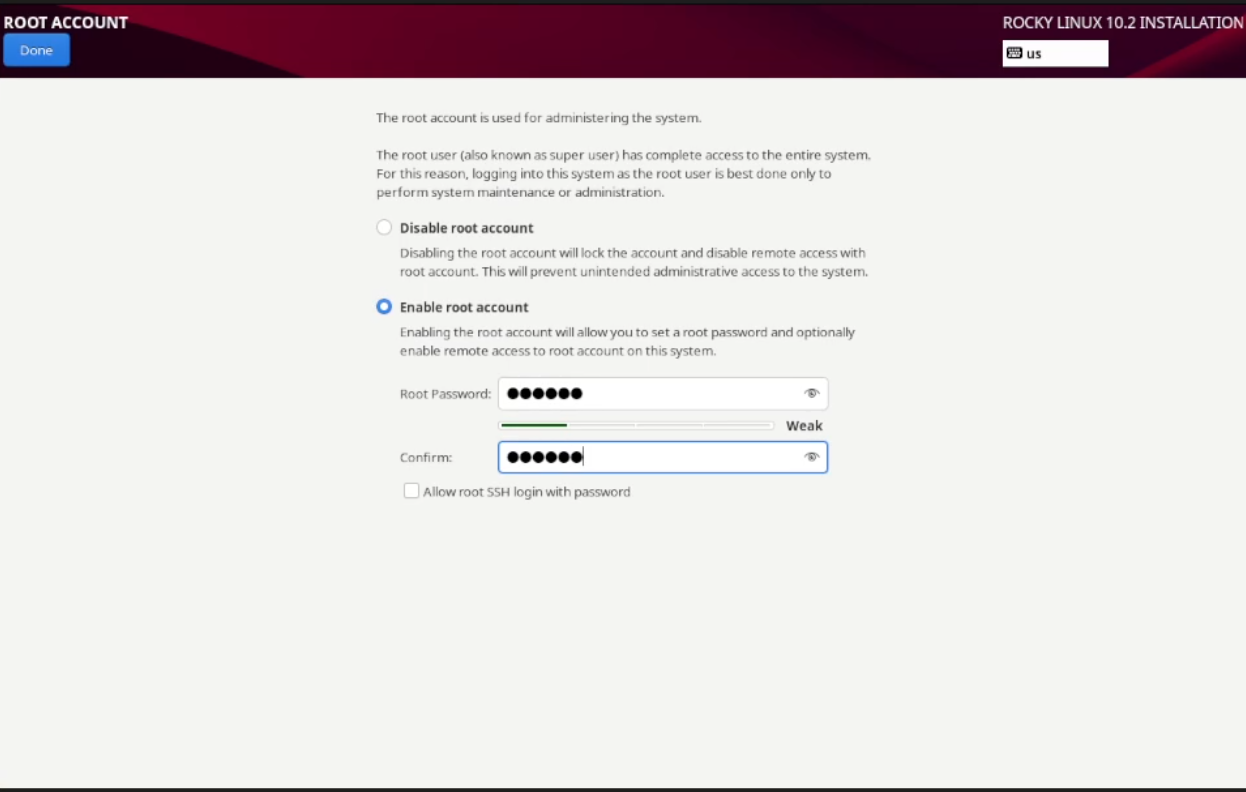
\includegraphics[width=0.7\linewidth,height=\textheight,keepaspectratio]{image/11.png}

}

\caption{\label{fig-011}Пароль для root}

\end{figure}%

Затем задаём локального пользователя с правами администратора и пароль
для него (рис.~\ref{fig-012})

\begin{figure}

\centering{

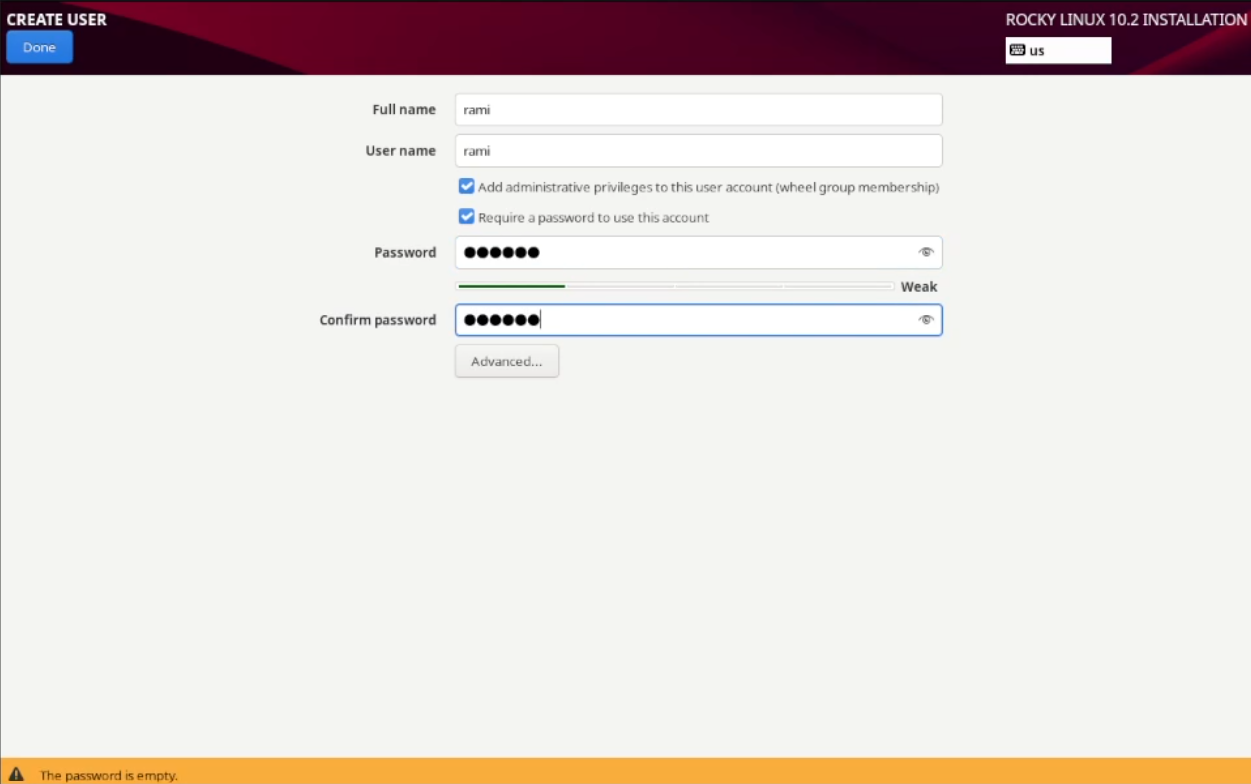
\includegraphics[width=0.7\linewidth,height=\textheight,keepaspectratio]{image/12.png}

}

\caption{\label{fig-012}Создание пользователя}

\end{figure}%

\begin{figure}

\centering{

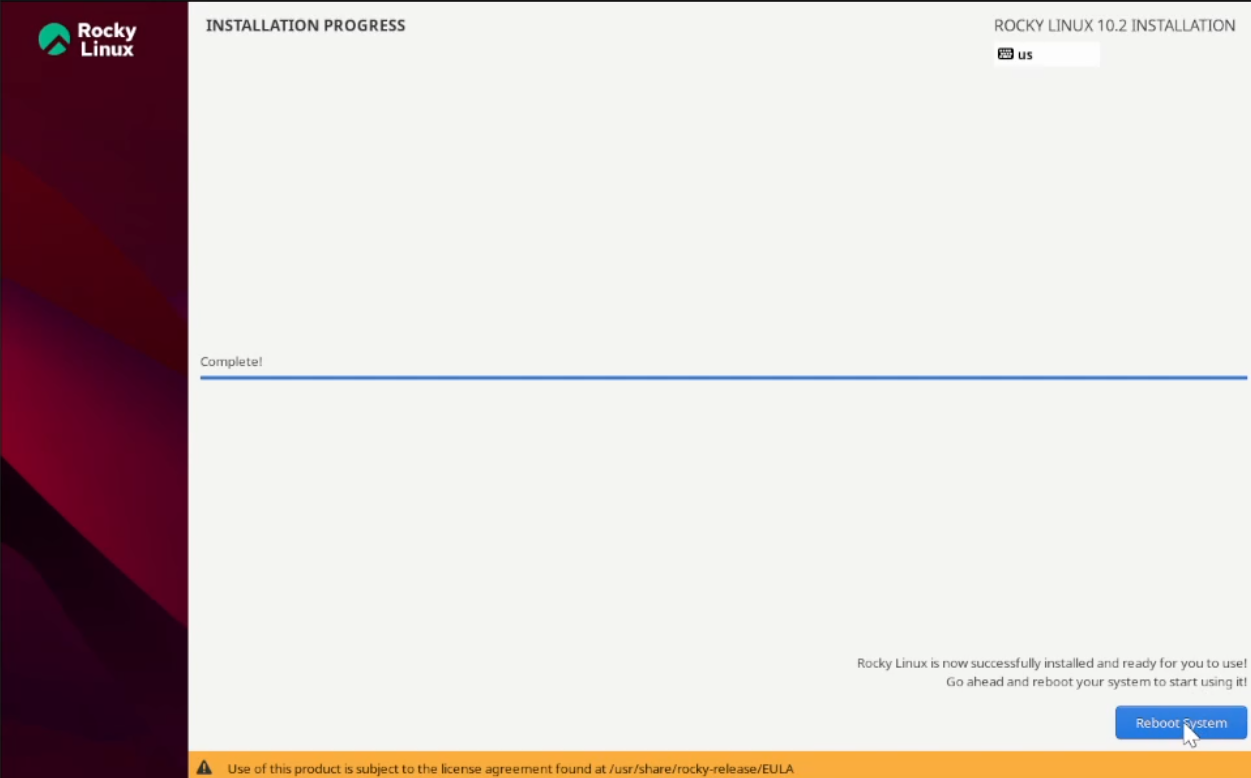
\includegraphics[width=0.7\linewidth,height=\textheight,keepaspectratio]{image/14.png}

}

\caption{\label{fig-014}Установка ОС}

\end{figure}%

\section{После
установки}\label{ux43fux43eux441ux43bux435-ux443ux441ux442ux430ux43dux43eux432ux43aux438}

Далее через терминал подключаем образ диска дополнений гостевой ОС:
(рис.~\ref{fig-015})

\begin{figure}

\centering{

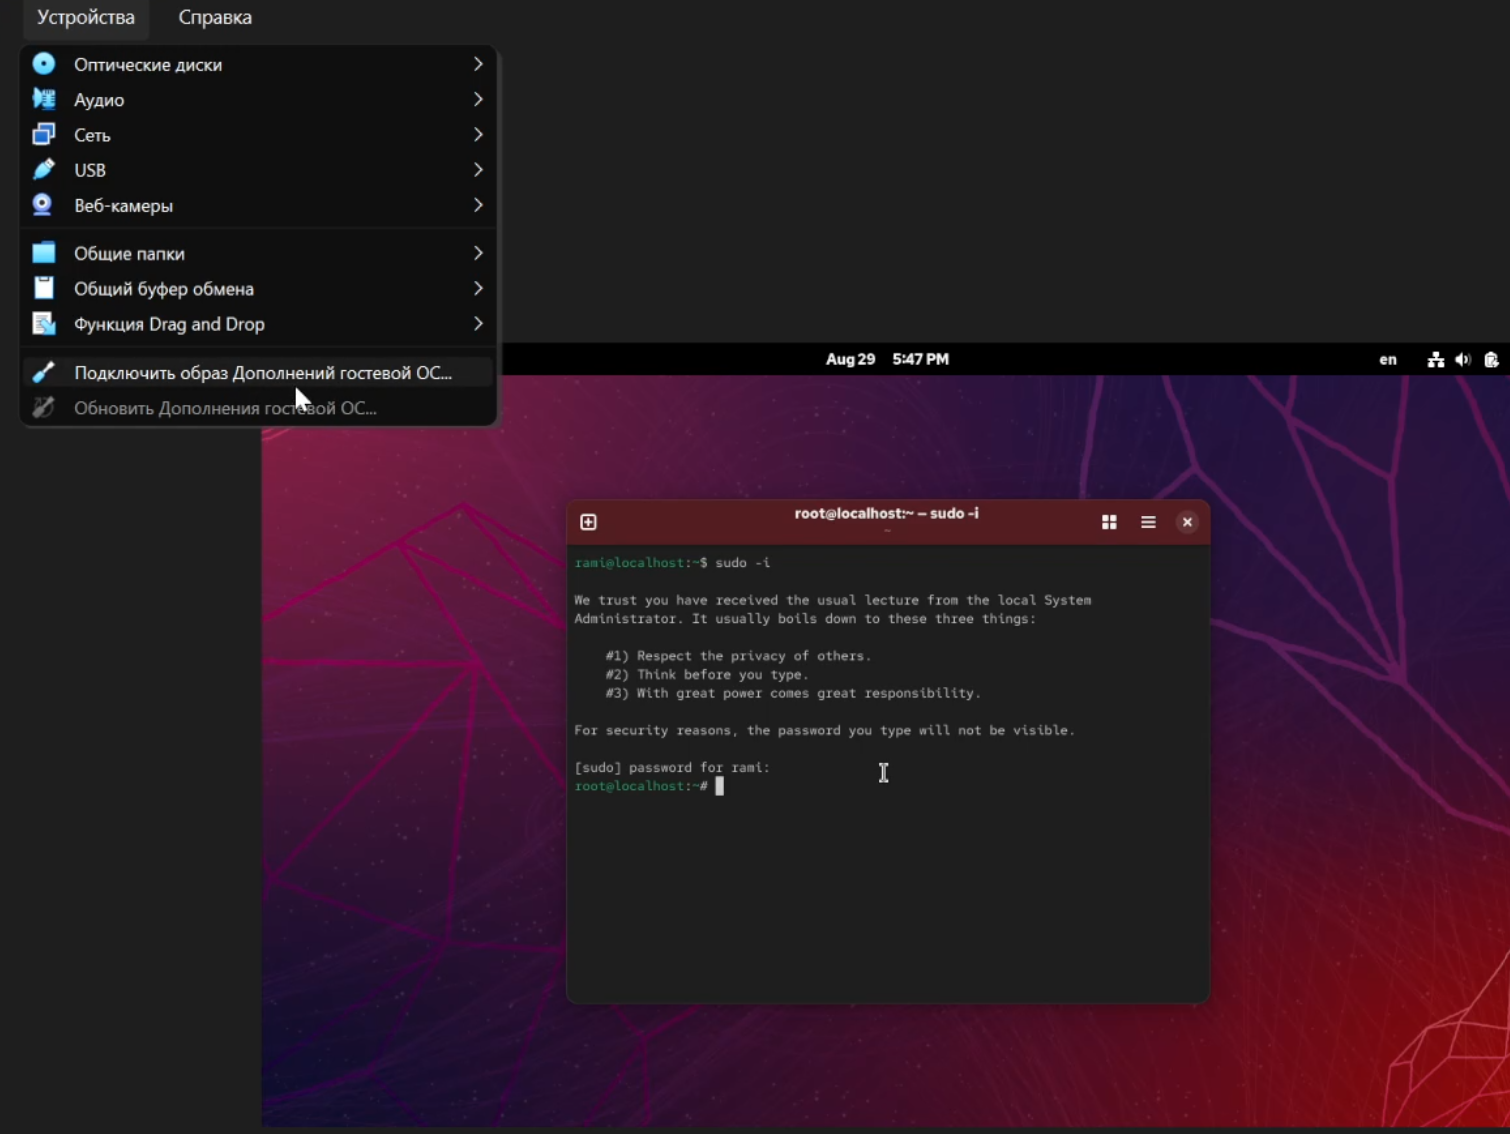
\includegraphics[width=0.7\linewidth,height=\textheight,keepaspectratio]{image/15.png}

}

\caption{\label{fig-015}Подключение образ диска дополнений гостевой ОС}

\end{figure}%

\chapter{Домашнее
задание}\label{ux434ux43eux43cux430ux448ux43dux435ux435-ux437ux430ux434ux430ux43dux438ux435}

\begin{enumerate}
\def\labelenumi{\arabic{enumi}.}
\tightlist
\item
  Версия ядра Linux (Linux version) (рис.~\ref{fig-018})
\item
  Частота процессора (Detected Mhz processor) (рис.~\ref{fig-019})
\item
  Модель процессора (CPU0) (рис.~\ref{fig-020})
\item
  Объем доступной оперативной памяти (Memory available)
  (рис.~\ref{fig-021})
\item
  Тип обнаруженного гипервизора (Hypervisor detected)
  (рис.~\ref{fig-022})
\item
  Тип файловой системы корневого раздела (рис.~\ref{fig-023})
\end{enumerate}

\begin{figure}

\centering{

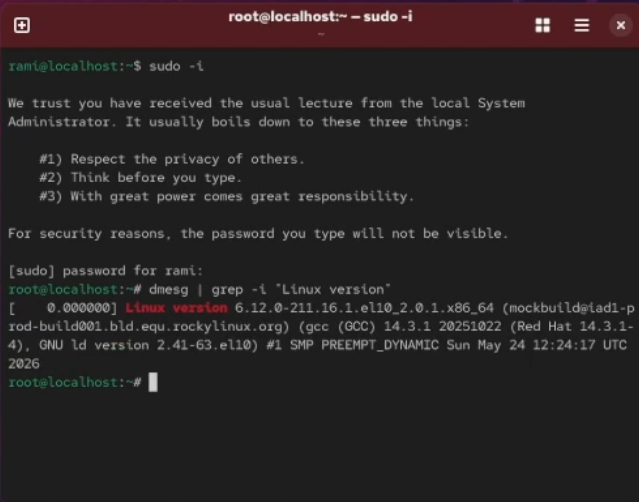
\includegraphics[width=0.7\linewidth,height=\textheight,keepaspectratio]{image/18.png}

}

\caption{\label{fig-018}Версия ядра Linux}

\end{figure}%

\begin{figure}

\centering{

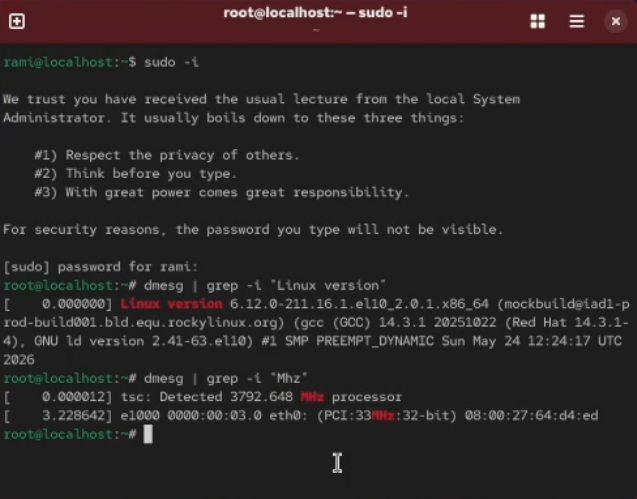
\includegraphics[width=0.7\linewidth,height=\textheight,keepaspectratio]{image/19.png}

}

\caption{\label{fig-019}Частота процессора}

\end{figure}%

\begin{figure}

\centering{

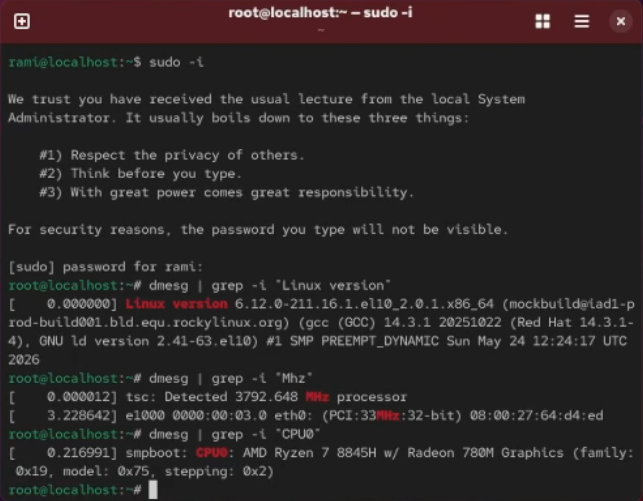
\includegraphics[width=0.7\linewidth,height=\textheight,keepaspectratio]{image/20.png}

}

\caption{\label{fig-020}Модель процессора}

\end{figure}%

\begin{figure}

\centering{

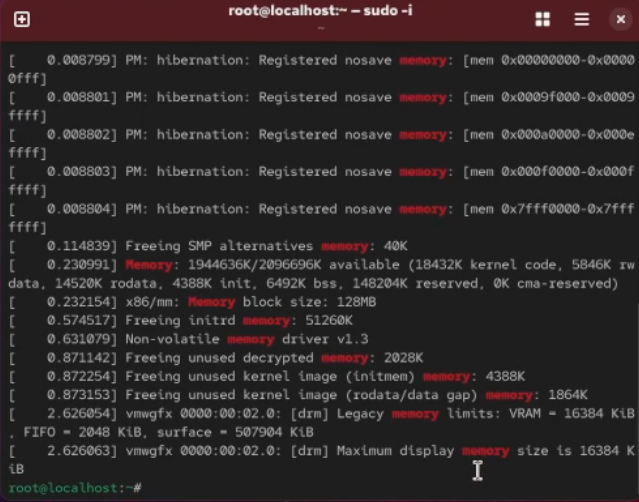
\includegraphics[width=0.7\linewidth,height=\textheight,keepaspectratio]{image/21.png}

}

\caption{\label{fig-021}Объем доступной оперативной памяти}

\end{figure}%

\begin{figure}

\centering{

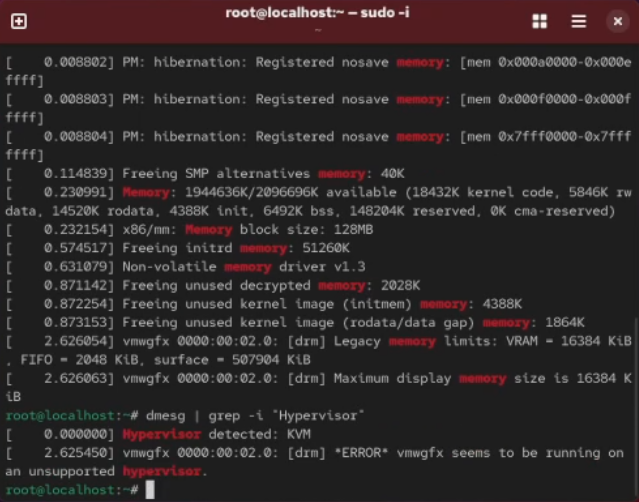
\includegraphics[width=0.7\linewidth,height=\textheight,keepaspectratio]{image/22.png}

}

\caption{\label{fig-022}Тип обнаруженного гипервизора}

\end{figure}%

\begin{figure}

\centering{

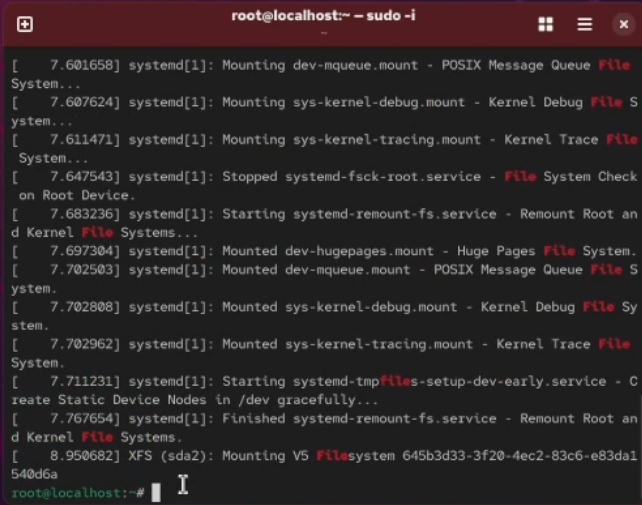
\includegraphics[width=0.7\linewidth,height=\textheight,keepaspectratio]{image/23.png}

}

\caption{\label{fig-023}Тип файловой системы корневого раздела}

\end{figure}%

\chapter{Контрольные вопросы +
ответы}\label{ux43aux43eux43dux442ux440ux43eux43bux44cux43dux44bux435-ux432ux43eux43fux440ux43eux441ux44b-ux43eux442ux432ux435ux442ux44b}

\begin{enumerate}
\def\labelenumi{\arabic{enumi}.}
\tightlist
\item
  Какую информацию содержит учётная запись пользователя?
\end{enumerate}

Учётная запись, как правило, содержит сведения, необходимые для
опознания пользователя при подключении к системе, сведения для
авторизации и учёта. Это идентификатор пользователя (login) и его
пароль.

\begin{enumerate}
\def\labelenumi{\arabic{enumi}.}
\setcounter{enumi}{1}
\tightlist
\item
  Укажите команды терминала и приведите примеры:
\end{enumerate}

\begin{itemize}
\item
  для получения справки по команде используют \emph{help}
\item
  для перемещения по файловой системе используют \emph{cd}
\item
  для просмотра содержимого каталога используют \emph{ls}
\item
  для определения объёма каталога используют \emph{du}
\item
  для создания/удаления каталогов используют \emph{mkdir/rmdir}, а для
  файлов \emph{touch/rm}
\item
  для задания определённых прав на файл/каталог используют \emph{chmod}
\item
  для просмотра истории команд используют \emph{history}
\end{itemize}

\begin{enumerate}
\def\labelenumi{\arabic{enumi}.}
\setcounter{enumi}{2}
\tightlist
\item
  Что такое файловая система? Приведите примеры с краткой
  характеристикой.
\end{enumerate}

Файловая система (англ. file system) --- порядок, определяющий способ
организации, хранения и именования данных во внешней памяти, и
обеспечивающий пользователю удобный интерфейс при работе с такими
данными. Простыми словами файловая система - это система хранения файлов
и организации каталогов. От файловой системы зависит, как файлы будут
кодироваться, храниться на диске и читаться компьютером.

Примеры:

\begin{itemize}
\item
  FAT (англ. File Allocation Table «таблица размещения файлов») ---
  классическая архитектура файловой системы, которая из-за своей
  простоты всё ещё широко применяется для флеш-накопителей. Используется
  в дискетах, картах памяти и некоторых других носителях информации.
  Ранее находила применение и на жёстких дисках.
\item
  NTFS (англ. new technology file system --- «файловая система новой
  технологии») --- стандартная файловая система для семейства
  операционных систем Windows NT фирмы Microsoft.
\item
  Ext4 (англ. fourth extended file system, ext4fs) --- журналируемая
  файловая система, используемая преимущественно в операционных системах
  с ядром Linux, созданная на базе ext3 в 2006 году.
\end{itemize}

\begin{enumerate}
\def\labelenumi{\arabic{enumi}.}
\setcounter{enumi}{3}
\tightlist
\item
  Как посмотреть, какие файловые системы подмонтированы в ОС?
\end{enumerate}

Следует ввести команду df.

\begin{enumerate}
\def\labelenumi{\arabic{enumi}.}
\setcounter{enumi}{4}
\tightlist
\item
  Как удалить зависший процесс?
\end{enumerate}

Чтобы удалить зависшй процесс, надо сначала узнать его PID с помощью
команды \emph{ps}. А после этого ввести \emph{kill }. И всё готово!

\chapter{Выводы}\label{ux432ux44bux432ux43eux434ux44b}

В ходе выполнения лабораторной работы мы приобрели практические навыки
установки операционной системы на виртуальную машину, настройки
минимально необходимых для дальнейшей работы сервисов.

\chapter*{Список
литературы}\label{ux441ux43fux438ux441ux43eux43a-ux43bux438ux442ux435ux440ux430ux442ux443ux440ux44b}
\addcontentsline{toc}{chapter}{Список литературы}

Лаборатораня работа №1 {[}Электронный ресурс{]}
URL:https:\{//esystem.rudn.ru/pluginfile.php/3096704/mod\_folder/content/0/001-lab\_virtualbox.pdf\}


\printbibliography



\end{document}
